% Options for packages loaded elsewhere
\PassOptionsToPackage{unicode}{hyperref}
\PassOptionsToPackage{hyphens}{url}
%
\documentclass[
]{book}
\usepackage{amsmath,amssymb}
\usepackage{lmodern}
\usepackage{iftex}
\ifPDFTeX
  \usepackage[T1]{fontenc}
  \usepackage[utf8]{inputenc}
  \usepackage{textcomp} % provide euro and other symbols
\else % if luatex or xetex
  \usepackage{unicode-math}
  \defaultfontfeatures{Scale=MatchLowercase}
  \defaultfontfeatures[\rmfamily]{Ligatures=TeX,Scale=1}
\fi
% Use upquote if available, for straight quotes in verbatim environments
\IfFileExists{upquote.sty}{\usepackage{upquote}}{}
\IfFileExists{microtype.sty}{% use microtype if available
  \usepackage[]{microtype}
  \UseMicrotypeSet[protrusion]{basicmath} % disable protrusion for tt fonts
}{}
\makeatletter
\@ifundefined{KOMAClassName}{% if non-KOMA class
  \IfFileExists{parskip.sty}{%
    \usepackage{parskip}
  }{% else
    \setlength{\parindent}{0pt}
    \setlength{\parskip}{6pt plus 2pt minus 1pt}}
}{% if KOMA class
  \KOMAoptions{parskip=half}}
\makeatother
\usepackage{xcolor}
\usepackage{longtable,booktabs,array}
\usepackage{calc} % for calculating minipage widths
% Correct order of tables after \paragraph or \subparagraph
\usepackage{etoolbox}
\makeatletter
\patchcmd\longtable{\par}{\if@noskipsec\mbox{}\fi\par}{}{}
\makeatother
% Allow footnotes in longtable head/foot
\IfFileExists{footnotehyper.sty}{\usepackage{footnotehyper}}{\usepackage{footnote}}
\makesavenoteenv{longtable}
\usepackage{graphicx}
\makeatletter
\def\maxwidth{\ifdim\Gin@nat@width>\linewidth\linewidth\else\Gin@nat@width\fi}
\def\maxheight{\ifdim\Gin@nat@height>\textheight\textheight\else\Gin@nat@height\fi}
\makeatother
% Scale images if necessary, so that they will not overflow the page
% margins by default, and it is still possible to overwrite the defaults
% using explicit options in \includegraphics[width, height, ...]{}
\setkeys{Gin}{width=\maxwidth,height=\maxheight,keepaspectratio}
% Set default figure placement to htbp
\makeatletter
\def\fps@figure{htbp}
\makeatother
\setlength{\emergencystretch}{3em} % prevent overfull lines
\providecommand{\tightlist}{%
  \setlength{\itemsep}{0pt}\setlength{\parskip}{0pt}}
\setcounter{secnumdepth}{5}
\usepackage{booktabs}
\ifLuaTeX
  \usepackage{selnolig}  % disable illegal ligatures
\fi
\usepackage[]{natbib}
\bibliographystyle{apalike}
\IfFileExists{bookmark.sty}{\usepackage{bookmark}}{\usepackage{hyperref}}
\IfFileExists{xurl.sty}{\usepackage{xurl}}{} % add URL line breaks if available
\urlstyle{same} % disable monospaced font for URLs
\hypersetup{
  pdftitle={RAP Workshop},
  pdfauthor={Data Science Team},
  hidelinks,
  pdfcreator={LaTeX via pandoc}}

\title{RAP Workshop}
\author{Data Science Team}
\date{2023-09-06}

\begin{document}
\maketitle

{
\setcounter{tocdepth}{1}
\tableofcontents
}
\hypertarget{rap-workshop}{%
\chapter{RAP Workshop}\label{rap-workshop}}

This document contains the examples and exercises for the DHSC Data Science RAP Workshop in R. This will take you through:

\begin{itemize}
\tightlist
\item
  Reading in data
\item
  Manipulating data
\item
  Plotting data
\item
  Calculating statistics
\end{itemize}

\hypertarget{intro-to-plotting-and-calculating-summary-statistics}{%
\chapter{Intro to plotting and calculating summary statistics}\label{intro-to-plotting-and-calculating-summary-statistics}}

This page will take you through the steps of reading, filtering and plotting data. We will then generate summary statistics. The next page is an exercise to test your knowledge.

\hypertarget{dataset-background}{%
\section{Dataset background}\label{dataset-background}}

To obtain the data needed for this exercise, we use the onsr package, which reads in data from the ONS using their API. For this section, we'll be using data regarding online job adverts.

ONS gives the following information on this dataset:

``Adzuna is an online job search engine who collate information from thousands of different sources in the UK. These range from direct employers' websites to recruitment software providers to traditional job boards thus providing a comprehensive view of current online job adverts.

Adzuna is working in partnership with ONS and have made data available for analysis including online advert job descriptions, job titles, job locations, job categories and salary information.

The data provided are a point-in-time estimate of all job adverts indexed in Adzuna's job search engine during the point of data extraction.

These indices are created based upon job adverts provided by Adzuna. This data includes information on several million job advert entries each month, live across the UK, broken down by job category and UK countries and English regions.''

\hypertarget{reading-in-the-data}{%
\section{Reading in the data}\label{reading-in-the-data}}

We start by reading in a selection of libraries, which are collections of pre-written code that we can use to perform tasks for us.

\begin{verbatim}
library(onsr)
library(dplyr)
library(stringr)
library(readr)
\end{verbatim}

These packages do the following:

\begin{itemize}
\tightlist
\item
  onsr: reading in data from the ONS API
\item
  dplyr: used to manipulate datasets
\item
  stringr: we will use to manipulate strings
\item
  readr: allows us to save a dataframe as a csv file
\end{itemize}

\begin{verbatim}
# read in info on ONS datasets and display
datasets <- ons_datasets()
print(datasets$id)

# select a dataset
job_ads <- ons_get(id = "online-job-advert-estimates")

# print columns
print(colnames(job_ads))

# print job types
print(unique(job_ads$AdzunaJobsCategory))
\end{verbatim}

We can then call the ons\_datasets function to read in various datasets. We then call the ons\_get() to select the job adverts data we want. From this, we can print the column names of the dataset to see what our data looks like. We are interested in the types of jobs presented in the dataset, so we print the unique values in the AdzunaJobsCategory column.

\hypertarget{filtering-data}{%
\section{Filtering data}\label{filtering-data}}

We will use the package dplyr to clean the data and filter for last year's Health and Social care jobs data. We remove rows where the value is NA and filter the job category and time columns. We can then extract week number as a number (using the stringr package) to allow plotting the data to be straightforward. Note, the ``v4\_1'' column is the index values we will look to plot later.

\begin{verbatim}
# remove NAs, filter by job category, filter to 2022
health_jobs <- job_ads %>%
  filter(!is.na(v4_1)) %>%
  filter(AdzunaJobsCategory == "Healthcare and Social care") %>%
  filter(Time == 2022)

# extract week number and sort by
health_jobs_sorted <- health_jobs %>%
  mutate(week_no = str_extract(Week, "[0-9]+")) %>%
  mutate(week_no = as.numeric(week_no)) %>%
  arrange(week_no)
\end{verbatim}

Once we have a cleaned dataset, we save as a csv.

\begin{verbatim}
# save data to csv
write_csv(
  health_jobs_sorted,
  file = "./output/health_jobs_data.csv"
\end{verbatim}

\hypertarget{plotting-data}{%
\section{Plotting data}\label{plotting-data}}

Now we will plot the data using the package ggplot2.

We read in the following packages:

\begin{verbatim}
library(readr)
library(ggplot2)
\end{verbatim}

We read in the csv we just created:

\begin{verbatim}
health_jobs_sorted = read_csv("./output/health_jobs_data.csv")
\end{verbatim}

Here we set up the plot - reading in DHSC colours, plotting a line of the index values and set the chart labels.

\begin{verbatim}
# plot

ggplot() +
  DHSCcolours::theme_dhsc() +
  geom_line(
    data = health_jobs_sorted,
    aes(week_no, v4_1, colour = AdzunaJobsCategory),
    linewidth = 1
  ) +
  theme(legend.position="none") +
  DHSCcolours::scale_colour_dhsc_d() +
  labs(
    title = "Healthcare and Social care job adverts",
    subtitle = "2022",
    x = "Week number",
    y = "Value")
\end{verbatim}

And save the plot

\begin{verbatim}
# save the plot
ggsave("./output/health_jobs_chart.svg",
         height = 5,
         width = 10,
         units="in",
         dpi=300)
\end{verbatim}

\begin{figure}
\centering
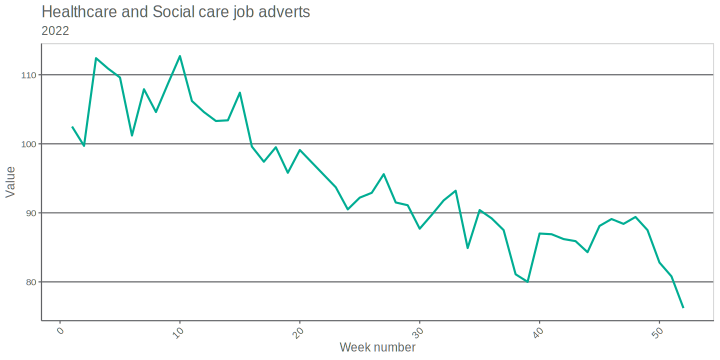
\includegraphics{health_jobs_chart.svg}
\caption{alt text}
\end{figure}

\hypertarget{generating-summary-stats}{%
\section{Generating summary stats}\label{generating-summary-stats}}

Finally, we will generate some summary statistics of the dataset.

We read in some now familiar packages:

\begin{verbatim}
library(readr)
library(dplyr)
\end{verbatim}

We read in the data:

\begin{verbatim}
health_jobs_sorted = read_csv("./output/health_jobs_data.csv")
\end{verbatim}

We calculate various stats:

\begin{verbatim}
# get stats

minimum <- min(health_jobs_sorted$v4_1)
maximum <- max(health_jobs_sorted$v4_1)
average <- mean(health_jobs_sorted$v4_1)
median <- median(health_jobs_sorted$v4_1)
\end{verbatim}

We then want to filter the dataset on the maximum and minimum values to find which week these occurred in. We start by creating a list where the now already defined variables for maximum and minimum are mapped to a string, which we can print in the output i.e.~set the max value to the string ``maximum''. We then loop over these values, retrieve the numerical value, filter on the dataset and pull the week number out. We then print these values along with the average and median already calculated.

\begin{verbatim}
stats = list("minimum" = maximum,
             "maximum"= minimum)

# get week values for stats, print

for (name in names(stats)) {
  stat_value = stats[[name]]

  week_no <- health_jobs_sorted %>%
    filter(v4_1 == stats[[name]]) %>%
    select(week_no) %>%
    pull

  print(paste("the ",name, "value is", stat_value, "(week:", week_no, ")"))
}

print(paste("the average value is",round(average,1)))
print(paste("the median value is",round(median)))
\end{verbatim}

This gives us some information about the dataset.

In the next section, you'll use these techniques to perform your own analysis on a different dataset.

\hypertarget{exercise}{%
\chapter{Exercise}\label{exercise}}

In this section, you will test your R skills by completing an exercise on the subjects covered on the previous page.

Please complete the following tasks:

\begin{enumerate}
\def\labelenumi{\arabic{enumi}.}
\item
  Download and clean the ONS data for Education job adverts in 2022.
\item
  Plot a time series chart for vacancies, using DHSC colours.
\item
  Establish which weeks had the lowest and highest index values respectively for teaching job adverts.
\item
  Calculate the median and mean index values for Education job adverts in 2022.
\end{enumerate}

  \bibliography{book.bib,packages.bib}

\end{document}
